\documentclass{article}

\usepackage{aligned-overset}
\usepackage{amsmath}
\usepackage{amssymb}
\usepackage[shortlabels]{enumitem}
\usepackage{genealogytree}
\usepackage{hyperref}
\usepackage[utf8]{inputenc}
\usepackage{mathtools}
\usepackage{pgfplots}
\usepackage{physics}
\usepackage{tikz}
\usetikzlibrary{positioning}
\usepackage{xcolor}
\definecolor{light-gray}{gray}{.9}

\author{Karsten Lehmann}
\date{WiSe 2020}
\title{Lineare Algebra I: Übungen - Blatt 1}

\begin{document}

\maketitle

\vfill

\newpage

\section*{Übung 1}

Bestimmen Sie, welche der folgenden Abbildungen injektiv, surjektiv bzw. bijektiv sind:

\begin{enumerate}[(i)]
\item $f_1 \colon \mathbb{Z} \to \mathbb{Z}, x \mapsto (x + 1)^8$ \\
  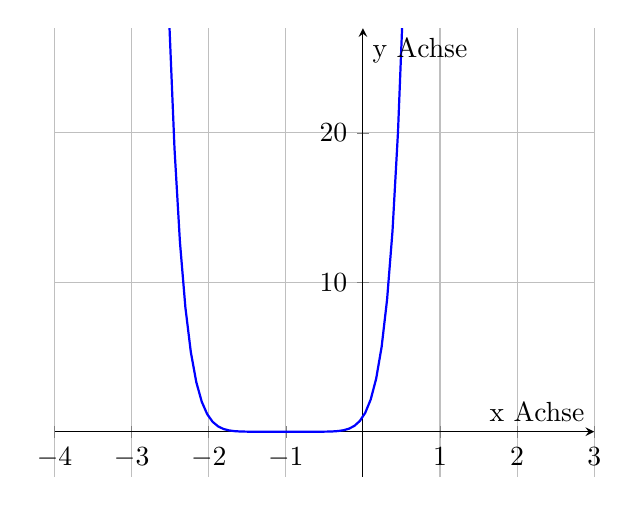
\begin{tikzpicture}
    \begin{axis}[
        axis x line=center,
        axis y line=center,
        domain=-4:3,
        grid=major,
        restrict y to domain=-1:30,
        samples=100,
        xlabel={x Achse},
        xmax=3,
        xmin=-4,
        ylabel={y Achse},
        ymax=27,
        ymin=-3,
      ]
      \addplot[blue, thick] { (x + 1) ^ 8 };
    \end{axis}
  \end{tikzpicture}

  \emph{Injektiv}: Widerspruchsbeweis, Annahme:
  \[
    \exists x_1, x_2 \in \mathbb{Z}, x_1 \ne x_2 \colon f_1(x_1) = f_1(x_2)
  \]

  Wenn $x_1 = -2$ und $x_2 = 0$, dann
  \[
    (x_1 + 1)^8 = (-2 + 1)^8 = (-1)^8 = 1 
  \]
  und
  \[
    (x_2 + 1)^8 = (0 + 1)^8 = 1^8 = 1
  \]

  Somit gilt $f_1(x_1) = f_1(x_2)$ für mindestens $x_1 = -2, x_2 = 0$. Damit kann $f_1$ nicht injektiv sein.

  \emph{Surjektiv}: Widerspruchsbeweis, Annahme: es existiert ein $y \in \mathbb{Z}$, welches nicht im Bild von
  $\mathbb{Z}$ unter $f_1$ enthalten ist.
  \[
    \exists y \in \mathbb{Z} \colon y \notin f_1(\mathbb{Z}) 
  \]

  Wenn $y = -1$, dann
  \begin{align*}
    y  &= (x + 1)^8 \\
    -1 &= (x + 1)^8 \\
    -1 &= ((x + 1)^4)^2 \\
    -1 \overset{\text{Substituiere } (x + 1)^4 \text{ mit } a}&{=} a^2 \\
  \end{align*}
  Das ist ein Widerspruch zu $a^2 \geq 0$, somit ist $y = -1$ nicht im Bild von $\mathbb{Z}$
  unter $f_1$ enthalten und $f_1$ ist auch nicht surjektiv.

  \emph{Bijektiv}: Eine Abbildung heißt bijektiv genau dann, wenn sie injektiv und surjektiv ist.
  Das $f_1$ wie oben gezeigt weder injektiv noch surjektiv ist, gilt $f_1$ ist nicht bijektiv.
  
\item $f_2 \colon \mathbb{N} \to \mathbb{N}, x \mapsto x^4$

  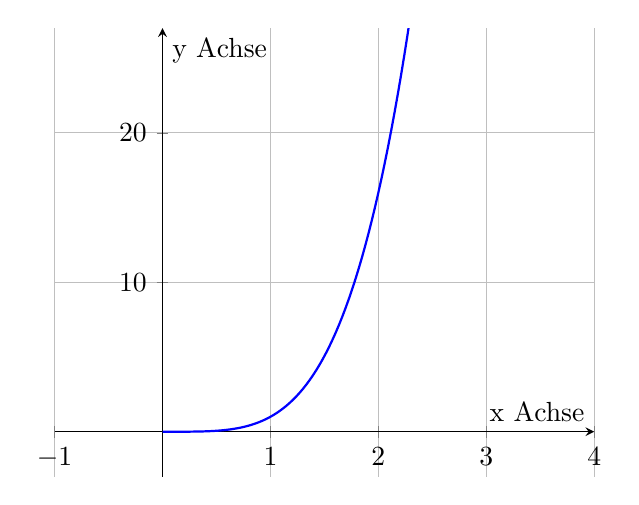
\begin{tikzpicture}
    \begin{axis}[
        axis x line=center,
        axis y line=center,
        domain=0:3,
        grid=major,
        restrict y to domain=-1:30,
        samples=100,
        xlabel={x Achse},
        xmax=4,
        xmin=-1,
        ylabel={y Achse},
        ymax=27,
        ymin=-3,
      ]
      \addplot[blue, thick] { x ^ 4 };
    \end{axis}
  \end{tikzpicture}

  \emph{Injektiv}:
  \begin{align*}
    n^4 - (n + 1)^4 &= n^4 - (n^4 + 2n + 1 \\
                    &= n^4 - n^4 - 2n - 1 \\
                    &= -2n - 1 \\
  \end{align*}
  Der Ausdruck $-2n -1$ ist kleiner als $0$ für alle $n \in \mathbb{N}$.
  Aus dem Trichotomiegesetz folgere ich nun, dass $(n + 1)^4 > n^4$.
  Somit gibt es keine zwei $n_1 \ne n_2 \in \mathbb{N}$ für die gilt: $f_2(n_1) = f_2(n_2)$.
  Damit ist $f_2$ injektiv.
  
  \emph{Surjektiv}: Widerspruchsbeweis, Annahme: es existiert ein $y \in \mathbb{N}$, welches nicht im Bild von
  $\mathbb{N}$ unter $f_2$ enthalten ist.
  \[
    \exists y \in \mathbb{N} \colon y \notin f_2(\mathbb{N}) 
  \]

  Wenn $y = 2$, dann
  \begin{align*}
    y  &= x^4 \\
    2 &= x^4 && | \sqrt[4]{()} \\
    \sqrt[4]{2} &= x \\
  \end{align*}
  $x = \sqrt[4]{2} \notin \mathbb{N}$, deswegen ist $f_2$ nicht surjektiv.
  
  \emph{Bijektiv}: Eine Abbildung heißt bijektiv genau dann, wenn sie injektiv und surjektiv ist.
  Da $f_2$ wie oben gezeigt nicht surjektiv ist, gilt $f_2$ ist nicht bijektiv.
  
\item $f_3 \colon \mathbb{R} \to \mathbb{R}, x \mapsto x^4 + 2$

  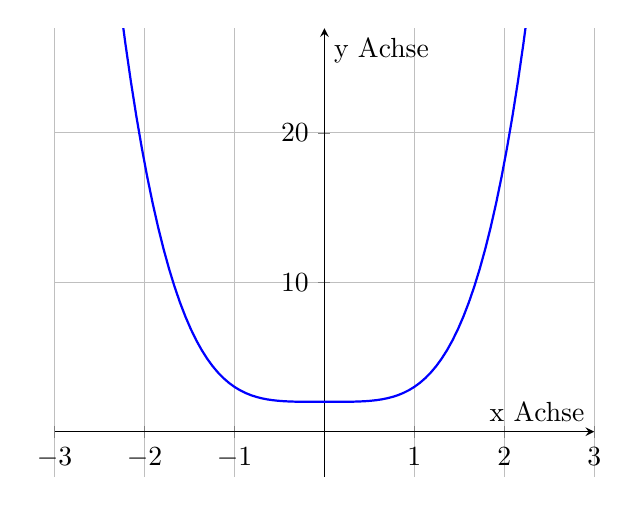
\begin{tikzpicture}
    \begin{axis}[
        axis x line=center,
        axis y line=center,
        domain=-3:3,
        grid=major,
        restrict y to domain=-1:30,
        samples=100,
        xlabel={x Achse},
        xmax=3,
        xmin=-3,
        ylabel={y Achse},
        ymax=27,
        ymin=-3,
      ]
      \addplot[blue, thick] { x ^ 4 + 2 };
    \end{axis}
  \end{tikzpicture}

  \emph{Injektiv}: Widerspruchsbeweis, Annahme:
  \[
    \exists x_1, x_2 \in \mathbb{R}, x_1 \ne x_2 \colon f_3(x_1) = f_3(x_2)
  \]

  Wenn $x_1 = -1$ und $x_2 = 1$, dann
  \[
    (x_1)^4 + 2 = (-1)^4 + 2 = 3  
  \]
  und
  \[
    (x_2)^4 + 2 = 1^4 + 2 = 3
  \]

  Somit gilt $f_3(x_1) = f_3(x_2)$ für mindestens $x_1 = -1, x_2 = 1$. Damit kann $f_3$ nicht injektiv sein.

  \emph{Surjektiv}: Widerspruchsbeweis, Annahme: es existiert ein $y \in \mathbb{R}$, welches nicht im Bild von
  $\mathbb{R}$ unter $f_3$ enthalten ist.
  \[
    \exists y \in \mathbb{R} \colon y \notin f_3(\mathbb{R}) 
  \]

  Wenn $y = 1$, dann
  \begin{align*}
    y  &= x^4 + 2 \\
    0  &= x^4 + 2 && | -2\\
    -2 &= x^4 \\
    -2 \overset{\text{Substituiere } x^2 \text{ mit } a}&{=} a^2 \\
  \end{align*}
  Das ist ein Widerspruch zu $a^2 \geq 0$, somit ist $y = 0$ nicht im Bild von $\mathbb{R}$
  unter $f_3$ enthalten und $f_3$ ist auch nicht surjektiv.

  \emph{Bijektiv}: Eine Abbildung heißt bijektiv genau dann, wenn sie injektiv und surjektiv ist.
  Das $f_3$ wie oben gezeigt weder injektiv noch surjektiv ist, gilt $f_3$ ist nicht bijektiv.

\item $f_4 \colon \mathbb{R} \to \mathbb{R}, x \mapsto x^7 + 15$

  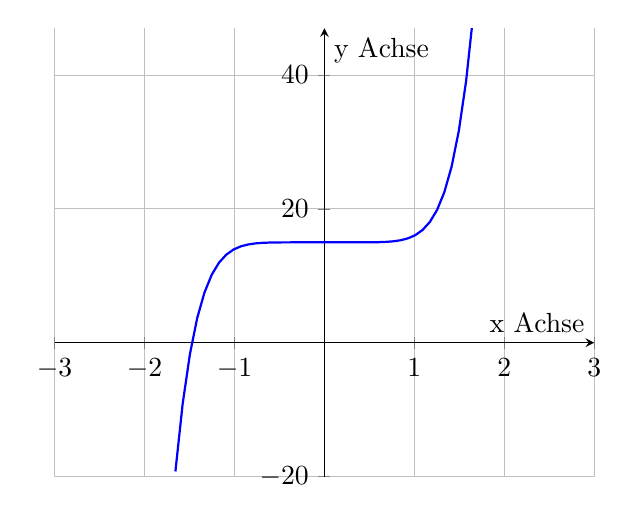
\begin{tikzpicture}
    \begin{axis}[
        axis x line=center,
        axis y line=center,
        domain=-4:4,
        grid=major,
        restrict y to domain=-30:50,
        samples=100,
        xlabel={x Achse},
        xmax=3,
        xmin=-3,
        ylabel={y Achse},
        ymax=47,
        ymin=-20,
      ]
      \addplot[blue, thick] { x ^ 7 + 15 };
    \end{axis}
  \end{tikzpicture}

  \emph{Injektiv}: Widerspruchsbeweis, angenommen $f_4$ ist nicht injektiv, dann existieren zwei
  $x_1 \ne x_2 \in \mathbb{R}$ für welche gilt: $f_4(x_1) = f_4(x_2)$.

  \begin{align*}
    (x_1)^7 + 15 &= (x_2)^7 + 15 && | -15 \\
    (x_1)^7      &= (x_2)^7      && | \sqrt[7]{(\ldots)} \\
    x_1          &= x_2 \\
  \end{align*}

  Somit ist $x_1 = x_2$ und dies ist ein Widerspruch zu der Annahme. Damit ist $f_4$ injektiv.

  \emph{Surjektiv}:

  \begin{align*}
    y                &= x^7 +  15 && | -15 \\
    y - 15           &= x^7      && | \sqrt[7]{(\ldots)} \\
    \sqrt[7]{y - 15} &= x
  \end{align*}

  Nach Schulwissen ist bekannt, das $\sqrt[7]{y - 15}$ für alle $y \in \mathbb{R}$ definiert ist.
  Somit existiert für jedes $y \in \mathbb{R}$ ein $x \in \mathbb{R}$ mit $f_4(x) = y$ und $f_4$ ist
  surjektiv.

  \emph{Bijektiv}: Eine Abbildung heißt bijektiv genau dann, wenn sie injektiv und surjektiv ist.
  Da $f_4$ wie oben gezeigt injektiv und surjektiv ist, gilt $f_4$ ist bijektiv.

\end{enumerate}

\section*{Übung 2}

\begin{enumerate}[(i)]
\item Die Definition einer Abbildung besagt, dass \textbf{jedem} Element aus $X$ \textbf{genau ein} Element aus $Y$
  zugeordnet wird.
  Das heißt für jedes Element aus $X$ gibt es $m$ verschiedene Möglichkeiten der Zuordnung.
  Somit kommen mit jedem weiteren Element in $X$ für jeden Vorhandene Kombination an Zuordnungen $m$
  neue Zuordnungen hinzu. \\

  Somit ist die Menge der Zuordnungen von $X \to Y$ mit $n$ Elementen in $X$ und $m$ Elementen in $Y$
  \[
    m^n
  \]

\item Um zu umgehen, dass einem Element aus $Y$ zwei Element aus $X$ zugeordnet werden, muss die Zahl der Elemente
  in $Y$ mindestens genau so groß wie die Zahl der Elemente in $X$ sein.

  \[
    m \geq n
  \]

  Weiterhin hat kann man das erste Element aus $X$ (hier $x_1$) $m$ verschiedenen Elementen aus $Y$ zuordnen.
  Das zweite Element aus $X$ (hier $x_2$) kann man dann allen Elemente aus $Y$ außer dem Element welches $x_1$
  zugeordnet wurde zuordnen, also $m - 1$ verschiedenen Elementen. \\

  $x_3$ kann man noch $m - 2$ Elementen zuordnen usw. Schließlich kann man das Element $x_n$ noch $m - n + 1$
  Elementen aus $Y$ zuordnen. \\

  Für den Sonderfall $m = n$ geht das ganze somit genau auf und es gibt
  \[
    m * (m - 1) * (m - 2) * \dots * (1) = m!
  \]
  Möglichkeiten der Zuordnung. \\

  Für den Fall $m > n$ kann man diese Kette ebenfalls aufschreiben:

  \[
    m * (m - 1) * (m - 2) * \ldots * (m - n + 1) 
  \]

  Im Vergleich dazu $m!$ für $m > n$

  \[
    m! = m * (m - 1) * (m - 2) * \ldots * (m - n + 1) * \color{red} (m - n) * (m - n - 1) * \ldots * 1
  \]

  Der Unterschied ist hier rot dargestellt und lässt sich als $(m - n)!$ schreiben.
  Die Lösung ist somit

  \[
    \frac{m!}{(m - n)!}
  \]
\end{enumerate}

\section*{Übung 3}

\begin{enumerate}[(1)]
\item $(i) \Rightarrow (ii)$
  
  Annahme $\abs{X} = n \in \mathbb{N}$. Dann soll folgen: Sei $f \colon X \to X$ surjektiv
  $\Rightarrow f \colon X \to X$ ist injektiv. \\

  \emph{Induktionsannahme}: Es gilt
  \[
    P(n) = (\text{Eine surjektive Abbildung einer $n$-elementigen Menge auf sich selbst ist injektiv})
  \]

  \emph{Induktionsanfang}: Für $n = 1$ ist diese Aussage wahr, da es von $\{ x_1 \}$ auf $\{ x_1 \}$ nur eine Abbildung gibt und diese ist bijektiv. \\

  \emph{Induktionsschritt}: Es wird angenommen, dass für $n$ die Abbildung $\{ x_1, \ldots, x_n \} \to \{ f(x_1), \ldots, f(x_n) \}$
  bijektiv ist.
  
  Für $n + 1$ existiert eine weitere Abbildung von
  $X \setminus \{ x_1, \ldots, x_n \}$ nach $X \setminus \{ f(x_1), \ldots, f(x_n) \}$. 
  Diese beiden Mengen umfassen jeweils ein Element und deren Abbildung aufeinander ist somit wie oben gezeigt ebenfalls bijektiv.
  
\item $(ii) \Rightarrow (iii)$ \\

  Annahme: $f \colon X \to X \text{ ist surjektiv} \iff f \colon X \to X \text{ ist injektiv}$
  \begin{itemize}
  \item $\Rightarrow$
    Sei $f \colon X \to X$ eine surjektive Abbildung. Dann ist $f$ auch injektiv. \\

    Angenommen $f$ wäre nicht injektiv, so existieren $x_1 \ne x_2, y \in X$ mit $f(x_1) = f(x_2) = y$.
    Da jedes Element aus dem Definitionsbereich genau einem Element aus der Zielmenge zugeordnet ist und
    die Zielmenge gleich dem Definitionsbereich ist, muss es somit ein $y \in X$ existieren, für welches
    kein $x \in X \colon f(x) = y$ existiert.
    Ein Widerspruch dazu, das $f$ surjektiv ist.
  \item $\Leftarrow$
    Sei $f \colon X \to X$ eine injektive Abbildung. Dann ist $f$ auch surjektiv. \\

    Angenommen $f$ wäre nicht surjektiv, so existieren $y \in X$ für welches kein $x \in X$ mit $f(x) = y$.
    existiert.
    Da jedes Element aus dem Definitionsbereich genau einem Element aus der Zielmenge zugeordnet ist und
    die Zielmenge gleich dem Definitionsbereich ist, muss es somit zwei Elemente aus dem Definitionsbereich geben,
    welche dem selben Element aus der Zielmenge zugeordnet sind, (es existieren $x_1, x_2, y \in X$, mit
    $f(x_1) = f(x_2) = y$).
    Ein Widerspruch dazu, das $f$ injektiv ist.    
  \end{itemize}
  
\item $(iii) \Rightarrow (i)$

  Wenn $f$ injektiv ist, dann wird jedem Element aus dem Definitionsbereich ein noch nicht vergebenes Element der Zielmenge
  zugeordnet.
  Da Definitionsbereich und Zielmenge hier identisch sind, gilt $\abs{f(X)} = \abs{X}$.
  Daraus folgt, dass $X$ endlich ist.
\end{enumerate}

Somit folgt aus $(i) \Rightarrow (ii)$, $(ii) \Rightarrow (iii)$ und $(iii) \Rightarrow (i)$

\[
  (i) \iff (ii) \iff (iii)
\]
\end{document}